\documentclass[handout]{ximera}

\title{Learning Ximera, part 2!}
\author{Hilary Freeman}



\begin{document}
\begin{abstract}
  This is my second place to get started.
\end{abstract}
\maketitle

\begin{tikzpicture}
\draw (0,0) --(2,-2);
\end{tikzpicture}

Ken wants to see xake!!!


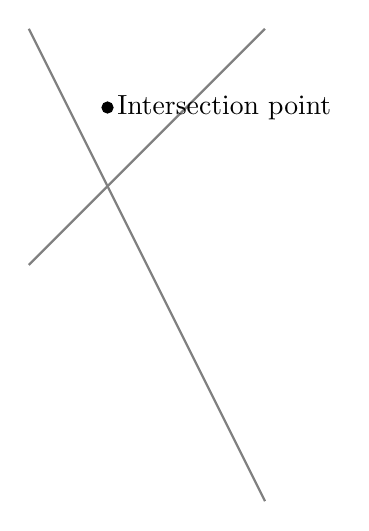
\begin{tikzpicture}
\draw[gray, thick] (-1,2) -- (2,-4);
\draw[gray, thick] (-1,-1) -- (2,2);
\filldraw[black] (0,1) circle (2pt) node[anchor=west] {Intersection point};
\end{tikzpicture}



\[
\graph{x^2}
\]

\end{document}
